\newpage
\subsection{[E] Removing an item from the list}
In order to remove an item from the list, just long click on the item that you want to remove. This will open the following popup showing the item's details.

\begin{figure}[H]
  \centering 
  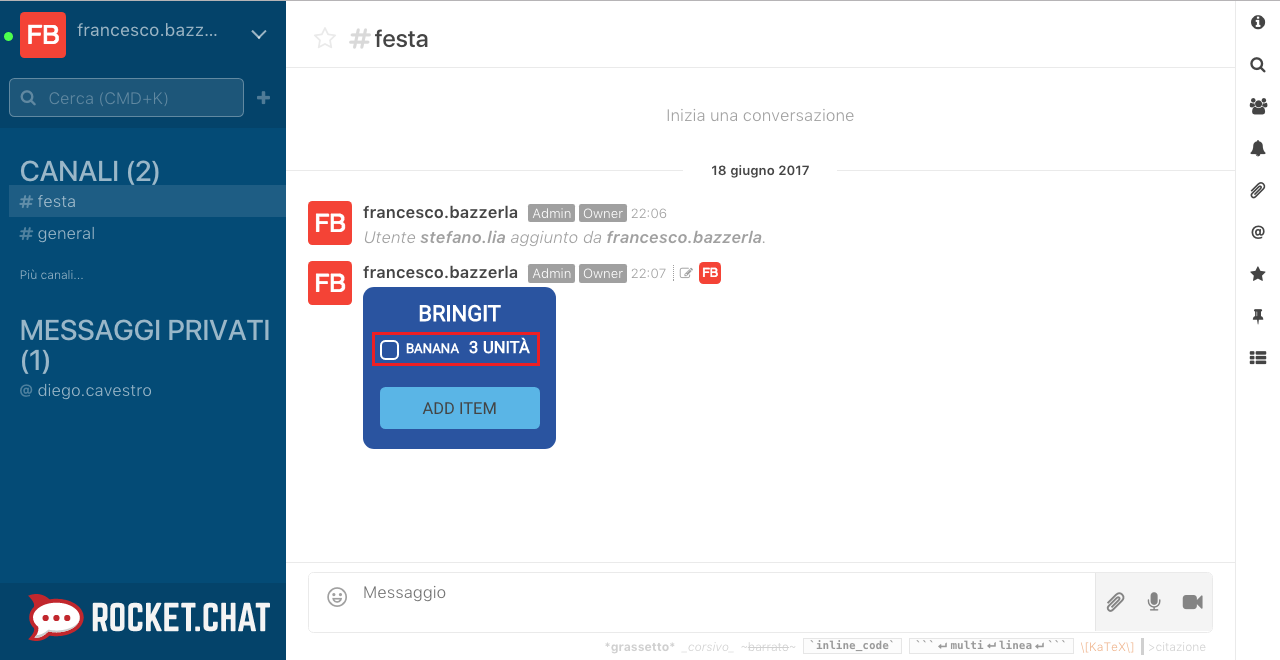
\includegraphics[width=\textwidth]{Sections/3-HowToUse/Images/bubble_item_to_delete.png}
  \caption{Popup showing the details of an item.}
\end{figure}

\begin{figure}[H]
  \centering 
  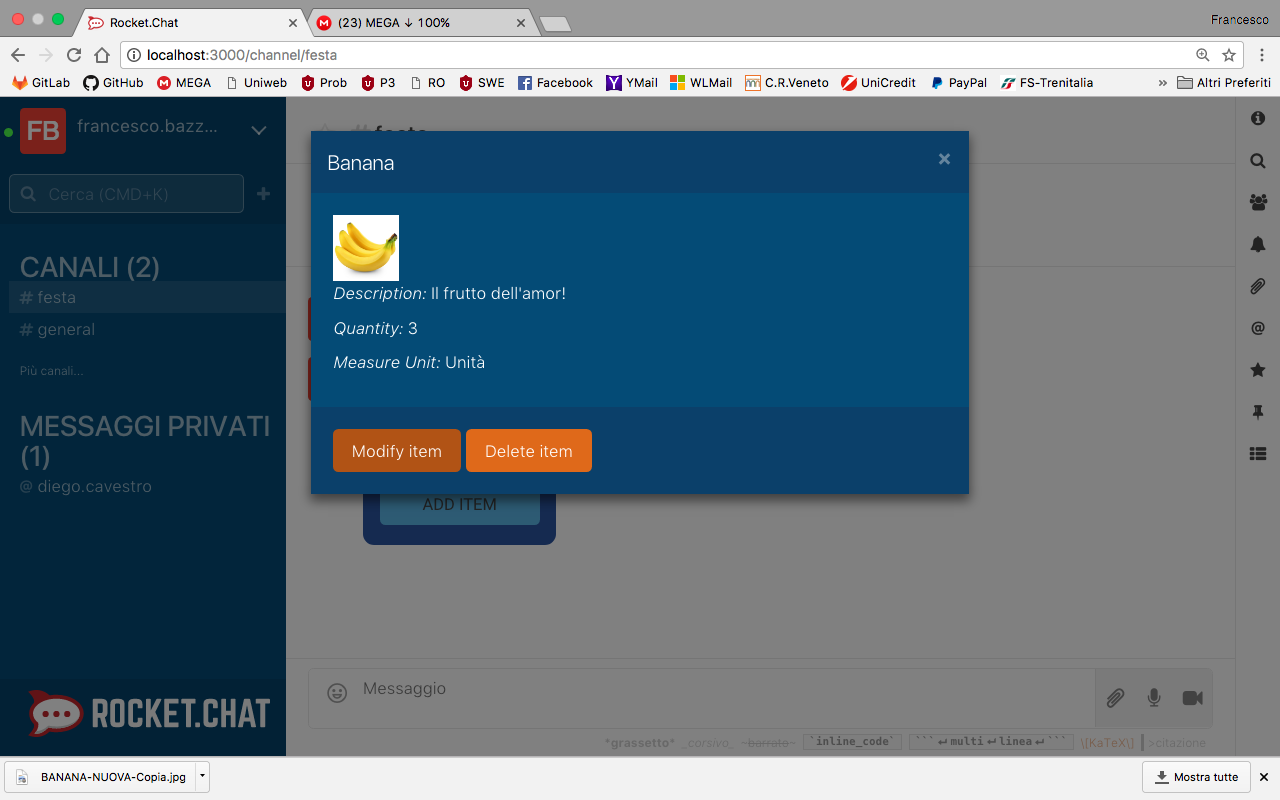
\includegraphics[width=\textwidth]{Sections/3-HowToUse/Images/item_details.png}
  \caption{Popup showing the details of an item.}
\end{figure}

To delete the item, just click on the \textit{"Delete"} button.

\begin{figure}[H]
  \centering 
  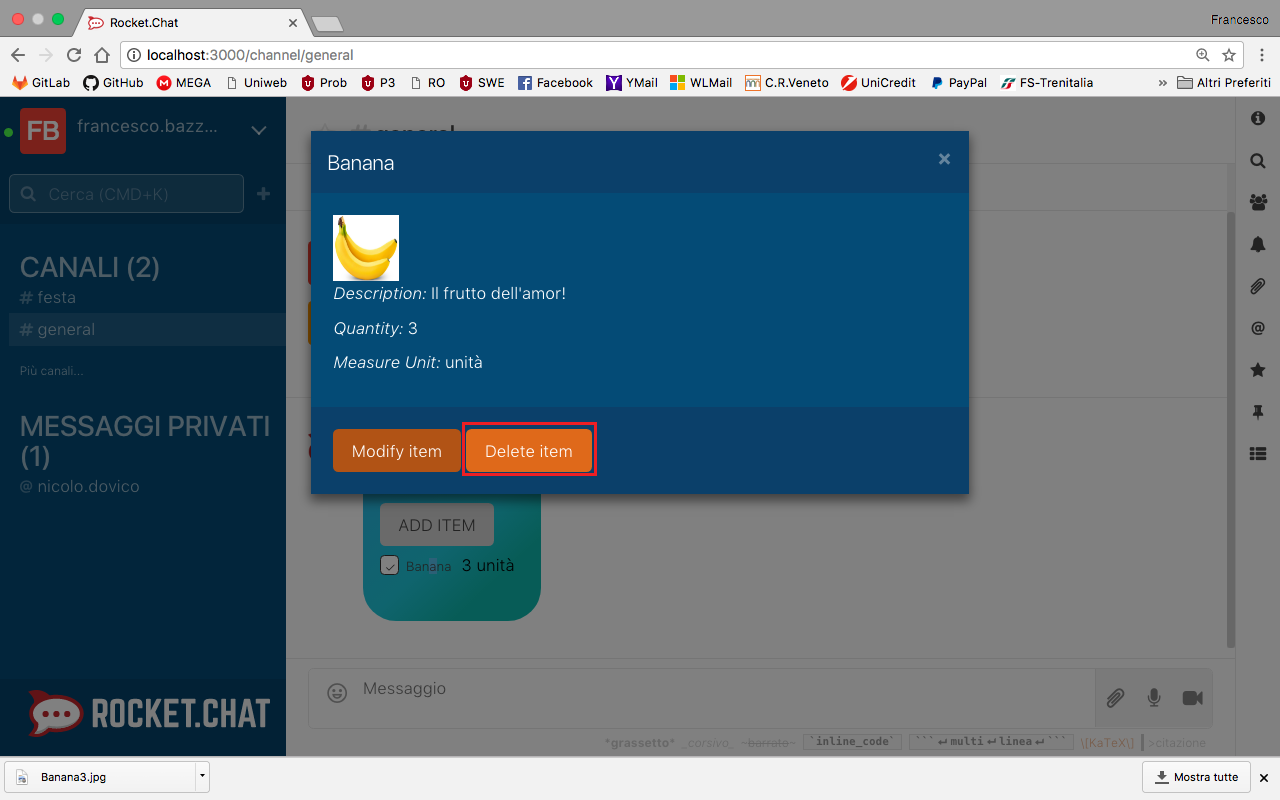
\includegraphics[width=\textwidth]{Sections/3-HowToUse/Images/popup_item_delete.png}
  \caption{Button to delete an item from a list.}
\end{figure}

\begin{figure}[H]
  \centering 
  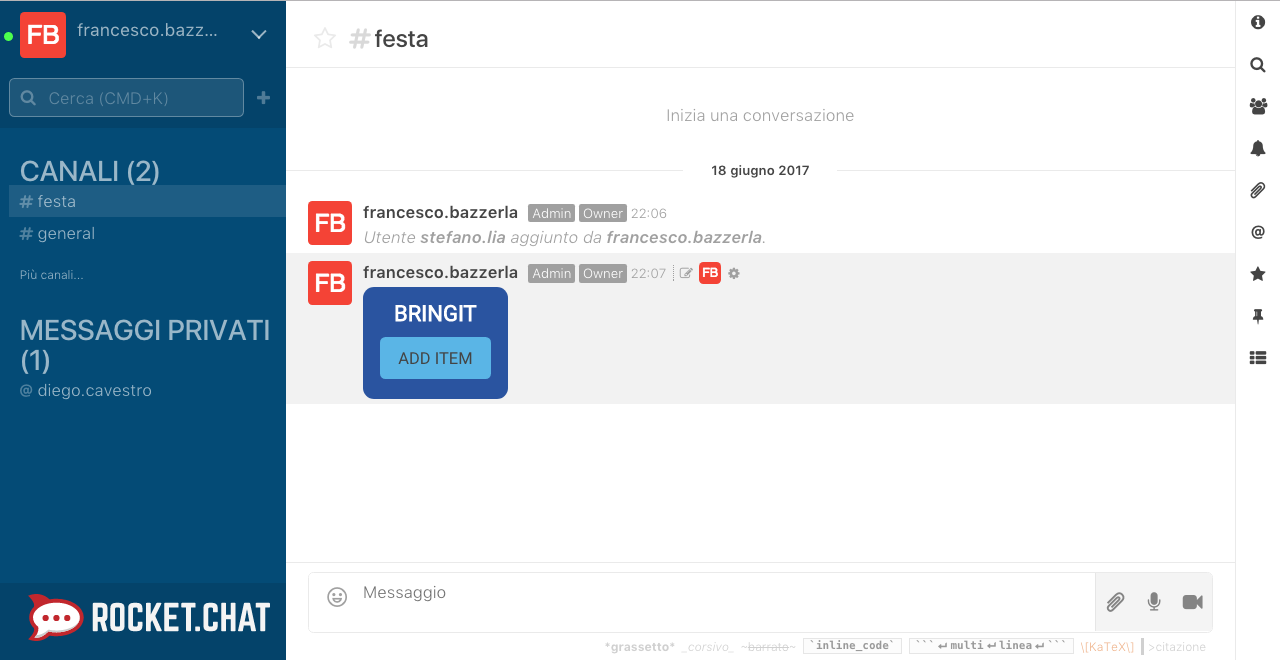
\includegraphics[width=\textwidth]{Sections/3-HowToUse/Images/item_deleted.png}
  \caption{Bubble with the deleted item.}
\end{figure}